\documentclass[twocolumn]{article}
\usepackage[utf8]{inputenc}
\usepackage{graphicx} %This lets you include images
\graphicspath{ {./} }
\usepackage{epstopdf} %This converts eps to pdf
\usepackage{caption} %Lets you write captions
\usepackage{amsmath} % math forumals
\usepackage{placeins} %Lets you use \FloatBarrier to prevent images and such from being places far away
\usepackage{hyperref} %Lets you include links in the doc that you can click and move you around. For example clicking a citation takes you to the bib
\usepackage{siunitx} % tables
\usepackage[
backend=biber,
style=alphabetic,
]{biblatex} % citation
\addbibresource{bibliography.bib} %Imports bibliography file
\usepackage{algorithm2e} % pseudo code
\usepackage{pdfpages}
\hypersetup{
colorlinks=true,
linkcolor=blue,
urlcolor=blue,
}

\setcounter{secnumdepth}{4}
%%%%%%%%%%%%%%%%%%%%%%%
\begin{document}
\title{Ant Colony Optimization}
\author{Jaraad Kamal}
\date{}
\maketitle
%%%%%%%%%%%%%%%%%%
\section{Introduction} \label{Intro}
The Traveling Salesman Problem (TSP) is a classic problem in 
computer science and mathematics. The task is to determine the optimal route/tour through a 
series of towns such that a salesman can visit all of them while minimizing the total distance 
traveled. The problem was first formally studied in the 1930s by Karl Menger. Historical records 
show that it was first mentioned in 1832 \cite{yu_2014}. 
This problem has major applications (one being 
postage and package delivery routes).

Traveling Salesman Problem is believed that determining an exact solution to the problem
cannot be completed in polynomial time.  All current methods of finding exact solutions 
to the problem require on the order of $\mathcal{O}(n!)$ computations where $n$ is
the number of towns \cite{yu_2014}. This makes it is infeasible to find an exact solution 
even for small values of $n$ such as $20$.

There are some methods to get an approximate solution very quickly. 
One such approach is Ant Colony Optimization. This approach 
developed by Dorigo and Gambardella in 1997 simulates a group of ants to 
determine a sufficient solution to TSP \cite{585892}. Sebastian Lague provides a 
beautiful visualization of this approach \cite{lague_2021}.

\section{Definitions}
Discussion of the algorithm requires the following definitions. A \textit{graph} is a series
of points (or towns) in a space. A \textit{vertex} is a particular point (or town) on this graph.
An \textit{edge} is a connection (or road) between two vertices on a graph. A \textit{cost} is 
the price (or distance) associated with a particular edge. Finally a \textit{path} (or tour) is a 
sequence of edges that visits different vertices on a graph without visiting the same one twice.


%%%%%%%%%%%%%%%%%%%
\section{Implementation} \label{Algos}
\subsection{Outline}
The basic approach for the algorithm is to simulate a number of ants that are scattered 
randomly along the graph and will randomly tour the graph. 

The decisions the ants makes are probabilistic. It will randomly choose an edge to follow but
will prefer edges with lower cost. In this sense the tour is ``semi-random" while also being a 
greedy algorithm because it prefers lowest cost at every step.

At the end of the first round of tours the ants will deposit a \textit{pheromone} along 
the path it took in its individual tour. The amount of \textit{pheromone} deposited depends on 
total cost of the ants path. Ants with lower total costs will deposit more pheromones
along each edge they crossed.

Then during the next round new ants will then semi-randomly tour the graph. However they will both
prefer cheaper edges as well as paths that have pheromones deposited on them. This helps reinforce 
``better" paths.

At the end of each round a portion of the pheromones will get \textit{evaporated} (i.e. a 
the amount of pheromones on each path will be reduced). This evaporation is to prevent paths from 
becoming permanent. Additionally, evaporation helps bad paths to fade out after multiple rounds.

\subsection{Notation}
There are a lot of variables and parameters that can be adjusted when implementing the algorithm.
For the sake of brevity I will define these as follows:
\begin{itemize}
    \item $m$ - The number of ants
    \item $a$ - The pheromone desirability weight, $a \ge 0$
    \item $b$ - The path desirability weight, $b \ge 1$
    \item $p$ - The pheromone evaporation factor, $0 < p < 1$
    \item $q$ - The pheromone deposition factor, $q > 0$
    \item $\eta_{xy}$ - The desirability of edge $(x,y)$. Typically inverse weight (e.g. $1/dist(x,y)$).
    \item $\tau_{xy}$ - The amount of pheromone on edge $(x,y)$
\end{itemize}
\subsection{Formulas}
\subsubsection{Edge Selection}
Let $U$ be the set of all vertices that have not been visited by the ant.

The probability an ant will travel from vertex $x$ to vertex $y$ (given $y \in U$):

\begin{align}
P_{xy} = \frac{(\tau_{xy})^a(\eta_{xy})^b}{\sum_{z \in U}^{}(\tau_{xz})^a (\eta_{xz})^b}
\end{align}
\cite{wikipedia_2022}

\subsubsection{Pheromone Update}
Let $l_k$ be the total cost of the tour of ant $k$.
I will define $\Delta\tau_{xy,k}$ as:
\begin{align}
    \Delta\tau_{xy,k} = 
    \begin{cases}
        q / l_k & \text{If ant } k \text{ traveled on edge } (x,y) \\
        0 & \text{Otherwise}
    \end{cases}
\end{align}

When updating the pheromones we can account for evaporation and new deposition at the 
same time with:
\begin{align}
    \tau_{xy} \gets (1 - p)\tau_{xy} + \sum_{k}^{m}\Delta\tau_{xy,k}    
\end{align}
\cite{wikipedia_2022}

\subsection{Thoughts and Modifications}
The one major difference between the algorithm and my implementation is in the 
determination of edge probabilities. During the first few rounds of the algorithm the pheromone strength ($\tau_{xy}$) on most of the edges is zero. Thus numerator of equation (1) is zero and there is no probability to explore a new edge. 
In my implementation I changed the probability equation by adding a constant to $\tau_{xy}$
to ensure a non-zero probability:

\begin{align}
P_{xy} = \frac{(1 + (\tau_{xy})^a)(\eta_{xy})^b}{\sum_{z \in U}^{}(1 + (\tau_{xz})^a) (\eta_{xz})^b}
\end{align}

After testing I found that the most significant factors are the pheromone evaporation factor,
pheromone desirability weight, and path desirability weight. The number of ants did not cause 
big changes. Results after using 5 ants and 20 ants were comparable. Additionally there are diminishing returns on the number of rounds/iterations. Running 500 iterations and 1000 iterations caused
little differences.

My default values are:

\begin{figure}[h]
\begin{tabular}{|c|S|}
    \hline
    m & {5 - 10}\\
    a & 2\\
    b & 5 \\
    p & 0.2 \\
    q & 5 \\
    \hline
\end{tabular}
\centering
\caption{Default values chosen for algorithm}
\label{fig:defaultVals}
\end{figure}

\subsection{Pseudo Code}

The algorithms are split into two major chunks. The first algorithm called Ant Brain
is the basic decision tree for each simulated ant. The second algorithm called Ant Optimize
will set up the ants each round and keep record/modify the pheromones. 

\RestyleAlgo{ruled}

%% This is needed if you want to add comments in
%% your algorithm with \Comment
\SetKwComment{Comment}{/* }{ */}
\SetAlgoLined

\begin{algorithm}[H]
\caption{Ant Brain}\label{alg:brain}
\KwData{$graph, pheromones$}
% \Comment{$\alpha path$}
\SetKwProg{Fn}{Function}{ :}{end}
\Fn{ant\_brain(G, PH: matrix, start: int)}{
    $path \gets \texttt{[]}$\;
    $visited \gets \texttt{\{}\}$ \Comment*[r]{set of visited nodes}
    $current \gets start$\;
    $cost \gets 0$\;
    \For{$i = 0, \dots, (n-2)$}{
        $weights \gets \texttt{[]}$\;
        \Comment{possible next locations}
        $choices \gets \{x | x \not \in visited\ \land x \not = start\}$\;
        \Comment{weights for weighted random choice}
        \For{$j \in choices$}{
            $\tau_j \gets \texttt{1/}G\texttt{[}current, j\texttt{]}$\;
            $\eta_j \gets PH\texttt{[}current, j\texttt{]}$\; 
            \Comment{a and b are predefined constants}
            $\texttt{append(}weights\texttt{, (1 + }\tau_j^a\texttt{) * }\eta_j^b\texttt{)}$\;
        }
        \Comment{weights should sum to 1}
        $weights \gets \frac{1}{\sum_{}^{}w_j}(weights)$\;
        \Comment{getting next node}
        $next \gets \texttt{random(}choices, weights\texttt{)}$\;
        \Comment{updating current, cost, path, and visited}
        $\texttt{append(}path, \texttt{(}current, next\texttt{))}$\;
        $cost \gets cost + G\texttt{[}current,next\texttt{]}$\;
        $visited \gets visited \cup \texttt{\{}next\texttt{\}}$\;
        $current \gets next$\;
        
    }
    \Comment{adding path back to start}
    $\texttt{append(}path, \texttt{(}current, start\texttt{))}$\;
    $cost \gets cost + G\texttt{[}current,start\texttt{]}$\;
    $\textbf{return} \texttt{(}cost,path\texttt{)}$\;
}

\end{algorithm}


\begin{algorithm}[H]
\caption{Ant Colony Optimization}\label{alg:colony}
\KwData{$graph$}
\SetKwProg{Fn}{Function}{ :}{end}
\Fn{ant\_optimize(G: matrix, num\_ants: int, num\_iter: int)}{
    $n \gets \texttt{size(}G\texttt{)}$\;
    \Comment{normalizing graph}
    $G \gets \texttt{(1/max(}G\texttt{))*}G$\;
    \Comment{Setting up pheromone matrix}
    $PH \gets \texttt{zeros((}n,n\texttt{))}$\;
    $ants \gets \texttt{[]}$\;
    \For {$i = 0,\dots,(num\_iter - 1)$}{
        \For {$a = 0,\dots,(num\_ants - 1)$}{
            $st \gets \texttt{randint(0,}n\texttt{ - 1)}$\;
            $\texttt{append(}ants\texttt{, ant\_brain(}G, PH, st\texttt{))}$\;
        }
        \Comment{Evaporating pheromones with predefined p}
        $PH \gets \texttt{(1 - }p\texttt{) * } PH$\;
        \Comment{Depositing new pheromones with predefined q}
        \For {$ant \in ants$}{
            $path \gets ant.path$\;
            $cost \gets ant.cost$\;
            \For {$step \in path$}{
                $(s, e) \gets step$\;
                \Comment{PH must be symmetric}
                $PH[s, e] \gets PH[s,e] + q\texttt{/}cost$\;
                $PH[e, s] \gets PH[e,s] + q\texttt{/}cost$\;
            }
        }
    }
    $best\_cost \gets \texttt{min(}ants\texttt{)}.cost$\;
    $best\_path \gets \texttt{min(}ants\texttt{)}.path$\;
    $\textbf{return} \texttt{(}best\_cost, best\_path\texttt{)}$\;
}

\end{algorithm}


%%%%%%%%%%%%%%%%%%%
\section{Results}
In order to test the algorithm I created a random map of 52 coordinates (Figure 2). Fifty-two coordinates
were chosen because it is large enough to be infeasible to obtain a an exact solution to TSP. 
\begin{figure}[h!]
\centering
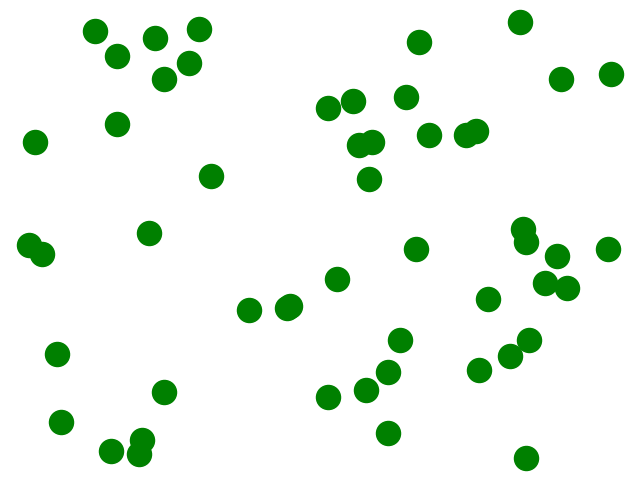
\includegraphics[width=\linewidth]{Ant_52_nodes_map.png}
\caption{
    Test map of points for Ant Colony Optimization. The average distance 
    between two points is 102.20 units.
}
\label{fig:map}
\end{figure}

I then ran the algorithm with 5 ants and 10 iterations (Figure 3) as well as 1000 
iterations (Figure 4) to see if there was any difference. After 10 iterations the 
solution had a total cost of 1595.23 units while the 1000 iteration solution had a 
cost of 1311.08 units. To visualize the ant decisions I plotted the pheromone trails left by the ants (Figure 5). 

\begin{figure}[h!]
\centering
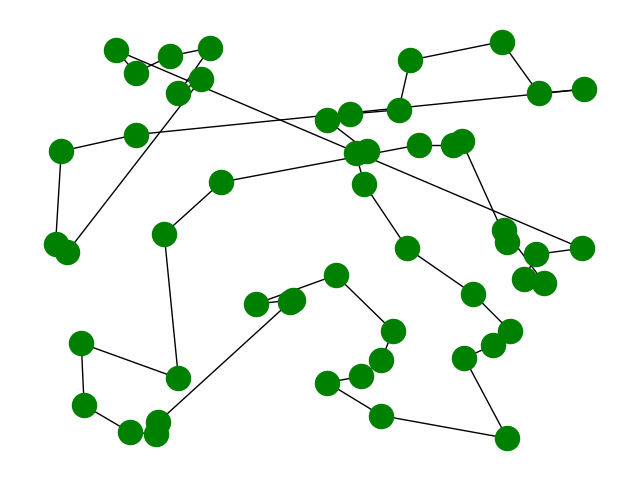
\includegraphics[width=\linewidth]{Ant_52_nodes_10_iterations.png}
\caption{
    Solution produced by 5 ants over 10 iterations. Total cost is
    1595.23 units. Time spent searching: 0.1 seconds.
}
\label{fig:tenItters}
\end{figure}

\begin{figure}[h!]
\centering
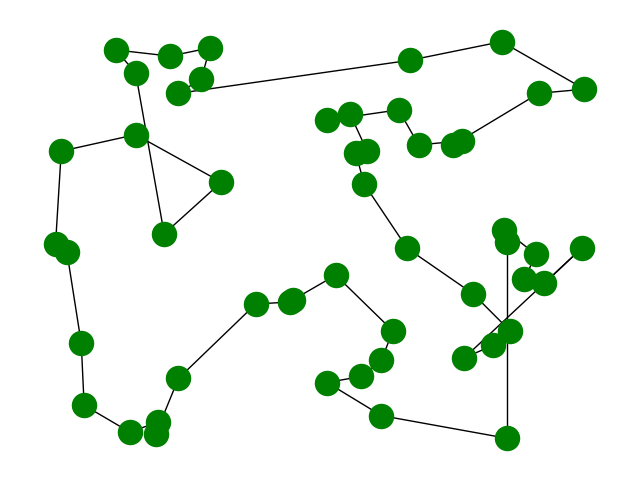
\includegraphics[width=\linewidth]{Ant_52_nodes_1000_iterations.png}
\caption{
    Solution produced by 5 ants over 10 iterations. Total cost is
    1311.08 units. Time spent searching: 8.6 seconds.
}
\label{fig:thousandItters}
\end{figure}

\begin{figure}[t!]
\centering
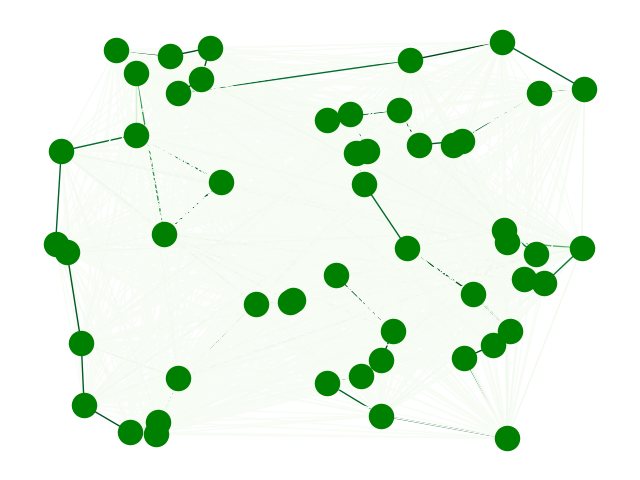
\includegraphics[width=\linewidth]{Ant_52_nodes_1000_iterations_pheromones.png}
\caption{
    Pheromone trails after 5 ants and 1000 iterations. The darker lines 
    represent edges that are more saturated with pheromones and thus more
    preferable to ants.
}
\label{fig:phermones}
\end{figure}

The figures show that the algorithm is finding a visually optimal path across all the 
vertices. There are big cycles to avoid unnecessary movement. Additionally, the second
iteration (which had 100x the rounds) did find a better solution. However upon close 
inspection the increased iterations only reduced the solution cost by 300 units. this is 
an indication of diminishing returns.

Overall the algorithm is very fast. As previously mentioned the TSP on a 52 vertex graph is 
computationally infeasible. This approach (with 1000 iterations) it only took 8.6 
seconds to compute.


%%%%%%%%%%%%%%%%%%%%
\section{Discussion}
The issue with this algorithm is that is probabilistic. Different runs of the algorithm can produce
slightly different results. There will also always be a probability that the given output is 
inefficient. However the greedy nature of each ant attempts to avoid this issue. 

Another issue is that there is no way to verify that a given output is THE solution to 
the traveling salesman problem on the graph. The only method is to compute the 
exact solution which is impossible for anything other than a tiny graph.

The absolute biggest benefit to this approach is that it is very fast. For larger graphs
this is incredibly fast than a true brute force approach. One of the only current methods
for finding a true solution to the graph is calculating each possible. This approach takes
around $\mathcal{O}(n!)$ computations where $n$ is the number of vertices \cite{yu_2014}. 
A graph of $52$ vertices (as in the example) would require $\mathcal{O}(52!)$ computations. 
To put the $52!$ into perspective, it is more than the number of seconds since the 
beginning of the universe \cite{nasa_2006}. Even for a graph with 10 
solutions an exact answer is infeasible to compute.

There are similar insect based algorithms. One such algorithm is called 
Bee Colony Optimization. This procedure attempts to simulate a swarm of bees in order to solve 
multi-dimensional optimization problems \cite{Karaboga2005ANIB}. While it does not solve the 
TSP like Ant Colony Optimization it uses a similar approach.

The benefit to Ant Colony Optimization is that approaches TSP in polynomial time. In the example
a solution to a 52 vertex graph was found in 8.6 seconds. 
An infeasible problem was given an approximate solution in a matter of seconds.
%%%%%%%%%%%%%%%%%%%%
\printbibliography
\includepdf[pages={-}]{code.pdf}
\end{document}
